Complex entity system..

\subsection{Entity System}
An Entity System consists of three main parts: Entities, Components and Systems.
An Entity is simply a label or identifier of an object. A Component is a pure data containers, and each entity has a collection of none to several different components. A System consist of logic for working with primarily one, but sometimes several, components. So, an object is an entity label and a collection of components that belong to it. The object is updated by different systems performing tasks on the components. A simple example used in this project is seen in figure \ref{fig:EntityComponentSystemExample}. 
\begin{figure}[H]
  \centering
  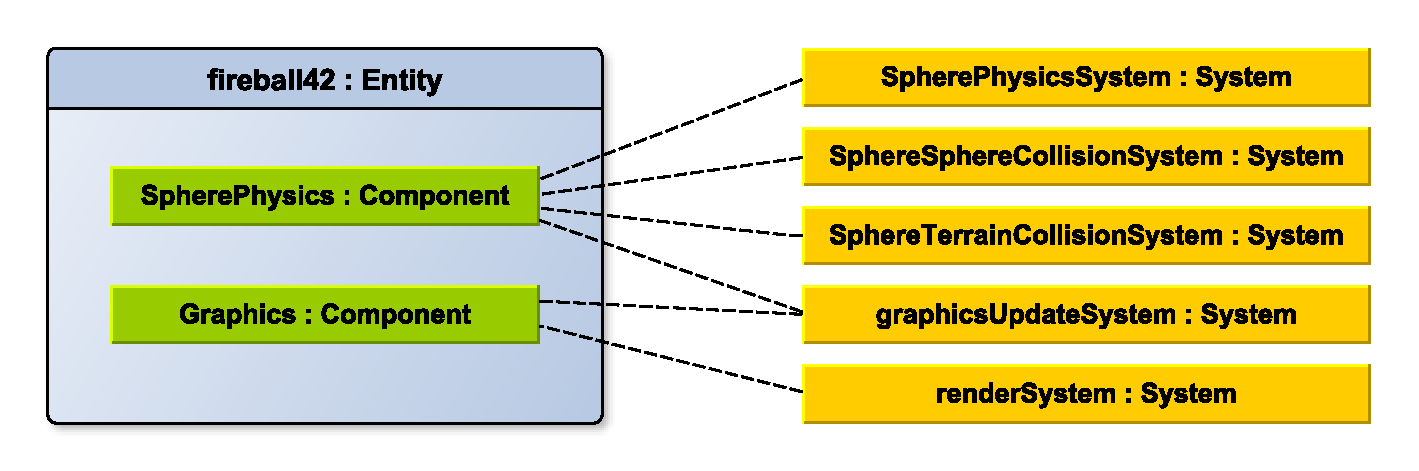
\includegraphics[width=0.9\linewidth]{images/EntityComponentSystemExample.eps}
  \caption{Caption}
  \label{fig:EntityComponentSystemExample}
\end{figure}
(TODO: reformulera och skriv nedan mer flytande och omarbetat)\\
* The idea behind: Systems perform on ALL components of a certain type, which is fetched from the EntityManager.\\
* Our system allows for components to require other components. This means that systems which work on multiple components can be proven to always work by fetching the component which require the others. The require check is performed at compile time and code is generated to handle the specific requirement-tree specified. The program writes part of itself to be maximum efficient and robust, by specifications by the developer in the source code.\\
* Easy to use (a natural work flow of what goes where and how to solve problems. minimal overhead to use the system), easy to maintain, easy to extend, extremely efficient, trivial to parallelize calculations, verifies consistency at compile time...

\subsection{Rendering}

\subsection{Physics}

